\section{Theoretical foundations}
\subsection{Historical background}
If one is to sketch the history exploring the weak interaction, 
the starting point is certainly the first formulation of the 
weak interaction, accomplished by Enrico Fermi in 1933. 
He described the nuclear beta decay as an interaction 
between four spin-$\frac{1}{2}$ particles at one vertex, 
introducing the neutrino. Although regarded highly speculative%
\footnote{His first attempt to publish was rejected by the journal
\emph{Nature} for this reason, triggering Fermi to abandon 
theoretical physics and turning to experiments for a while.}, 
it proofed to be useful for physics up at low energies. 
Soon it became clear that this approximation would not work out 
at high energies, where an interaction along an intermediate 
vector boson has to be included into the description. 
Experimentalists had a hard time dealing with this problem, 
as the involved particles do not form bound states (like the 
pions, mediating the interaction in nucleons). A first theory
on weak interaction, written by Glashow, Weinberg and Salam 
in 1968, identified three vector bosons: two charged $W$ bosons 
and a neutral $Z$ boson. A formula for their masses involved a 
parameter $\theta_W$ to be measured. In 1982, this empirical 
input allowed to calculate the masses up to
\begin{equation}
    M_W = 82 \pm 2 \mathrm{GeV / c^2},\qquad 
    M_Z = 92 \pm 2 \mathrm{GeV / c^2}
\end{equation}
The following year finally yielded the first confirmation 
of the existence of $W$ and $Z$ bosons, reported by the group 
of Carlo Rubbia at CERN\@.

\subsection{Short Overview to Quantum Field Theory}
\label{sub:qft}

The purpose of this section is to remind the reader about some basic Quantum field theory in order to prepare the 
more technical evaluation of the experiment\footnote{The introduction will not be exhaustive for the reader unfamiliar to
Quantum field theory. For a complete theoretical foundated introduction, please refer to \cite{schroeder} or
\cite{weinberg1996quantum}.} Our goal is to list all contributions to the process $e^{+}e^- \rightarrow f^+ f^-$ (see figure
\ref{fig:eemumu} for the first order contribution) with fermions $f$, since this is the key process of our experiment. 
\begin{figure}[htpb]
    \centering
    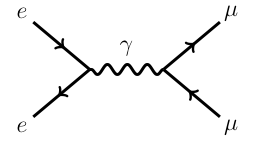
\includegraphics[width=0.6\linewidth]{figures/eemumu}
    \caption{Feynmandiagram of the first order contribution of $e^{+}e^- \rightarrow f^+ f^-$. Higher order will include
loops and interactions with the vacuum.}
    \label{fig:eemumu}
\end{figure}
The interesting observable in scattering is outgoing flux of particles scattered in a solid angle element $d\Omega$, divided
by the total incoming particle flux, this is called \textbf{differential crosssection}:
\begin{equation}
    \frac{d\sigma}{d\Omega} = \frac{\text{Scattered particle flux in }d\Omega }{\text{Total particle flux}}
\end{equation}
the total \textbf{cross section} $\sigma$  is obtained
by integrating over the angles $\theta$ and $\phi$ in polar coordiantes. This is dependent on the total momentum
of the incoming and outgoing particles. Let us formalize this intuition: 
\begin{equation}
    \sigma \sim \int_{\mathbb{R}^4} |\mathcal{M}|^2 \delta^4(p_1 + p_2 - p_3 - p_4) 
    \delta(p_3 ^2 - m_3^2 c^2) \delta(p_4 ^2 - m_4^2 c^2) d^4p_3 d^4p_4
    \label{eq:sigma}
\end{equation}
In words this means that we look at all processes which fullfill momentum and energy conservation, summing them up by
their probability. In fact this will be our method of operation in the end: Summing up particles numbers of the most important
contributions. The probabilities $|\mathcal{M}|^2$  have to be calculated in terms of the dirac equation.
Here we are only interested, how the $Z_0$ gauge boson couples to the different fermions, in order to calculate their
frequency. Let us now look at the matrix element $\mathcal{M}$ of incoming particles (\textbf{i}nitial)
with respect to outgoing particles (\textbf{f}inal):
\begin{equation}
    \mathcal{M}_{if} = \sqrt{2} G_F M_Z^2 \cdot j_\mu^{i} \cdot \frac{1}{s - M_Z^2 + iM_Z \Gamma_Z} \cdot j_\mu^{f}
    \label{eq:Mif}
\end{equation}

with the coupling $\sqrt{2} G_F M_Z^2$, the currents $j_\mu$ and the propagator
\begin{equation}
\frac{1}{s - M_Z^2 + iM_Z \Gamma_Z}.
\label{eq:propagator}
\end{equation}
If we only look at a particular process $e^{+}e^- \rightarrow Z^0 \rightarrow f^+ f^-$ we can express the partial crossection
by plugging in \eqref{eq:Mif} into  \eqref{eq:sigma} (and some calculations, which will not be shown here):
\begin{equation}
    \label{eq:breitwigner}
    \sigma_f = \frac{1}{M_Z^2} \frac{12\pi s \Gamma_i \Gamma_f }{(s- M_Z^2)^2 + M_Z^2 \Gamma_Z^2}
\end{equation}
This curve is named the \textit{Breit-Wigner distribution} and arises often from propagators of unstable particle as in 
\eqref{eq:propagator}. The maxima of the different curves depend on the respective fermion with 
partial decay widths $\Gamma_f$. As one is to accept this formulas arising from QFT calculations, one has to bear in mind
that these are only first-order processes, and as to far to be considered as approximations. Furthermore we can write down
the specific partial decay widths, which are dependent on the respective charge $Q_f$ of the fermion:
\begin{equation}
    \label{eq:gamma_f}
    \Gamma_f = \frac{G_F M_Z^3}{24 \sqrt{2} \pi} \left[ 1 + (1 - 4 |Q_f| \sin^2 \theta_W )^2 \right]
\end{equation}
The angle $\theta_W$ arising here is coming from the electro-weak unification.
\subsection{Strong Interaction}
\label{sub:strong}
As the overwhelming proportion of the particles observed will be hadronic and hence of quark origin, we need to have a short
look at the strong interaction responsible for the branching ratio (see figure~\ref{fig:hadrons} for an example of one 
Feynman diagram).
\begin{figure}[htpb]
    \centering
    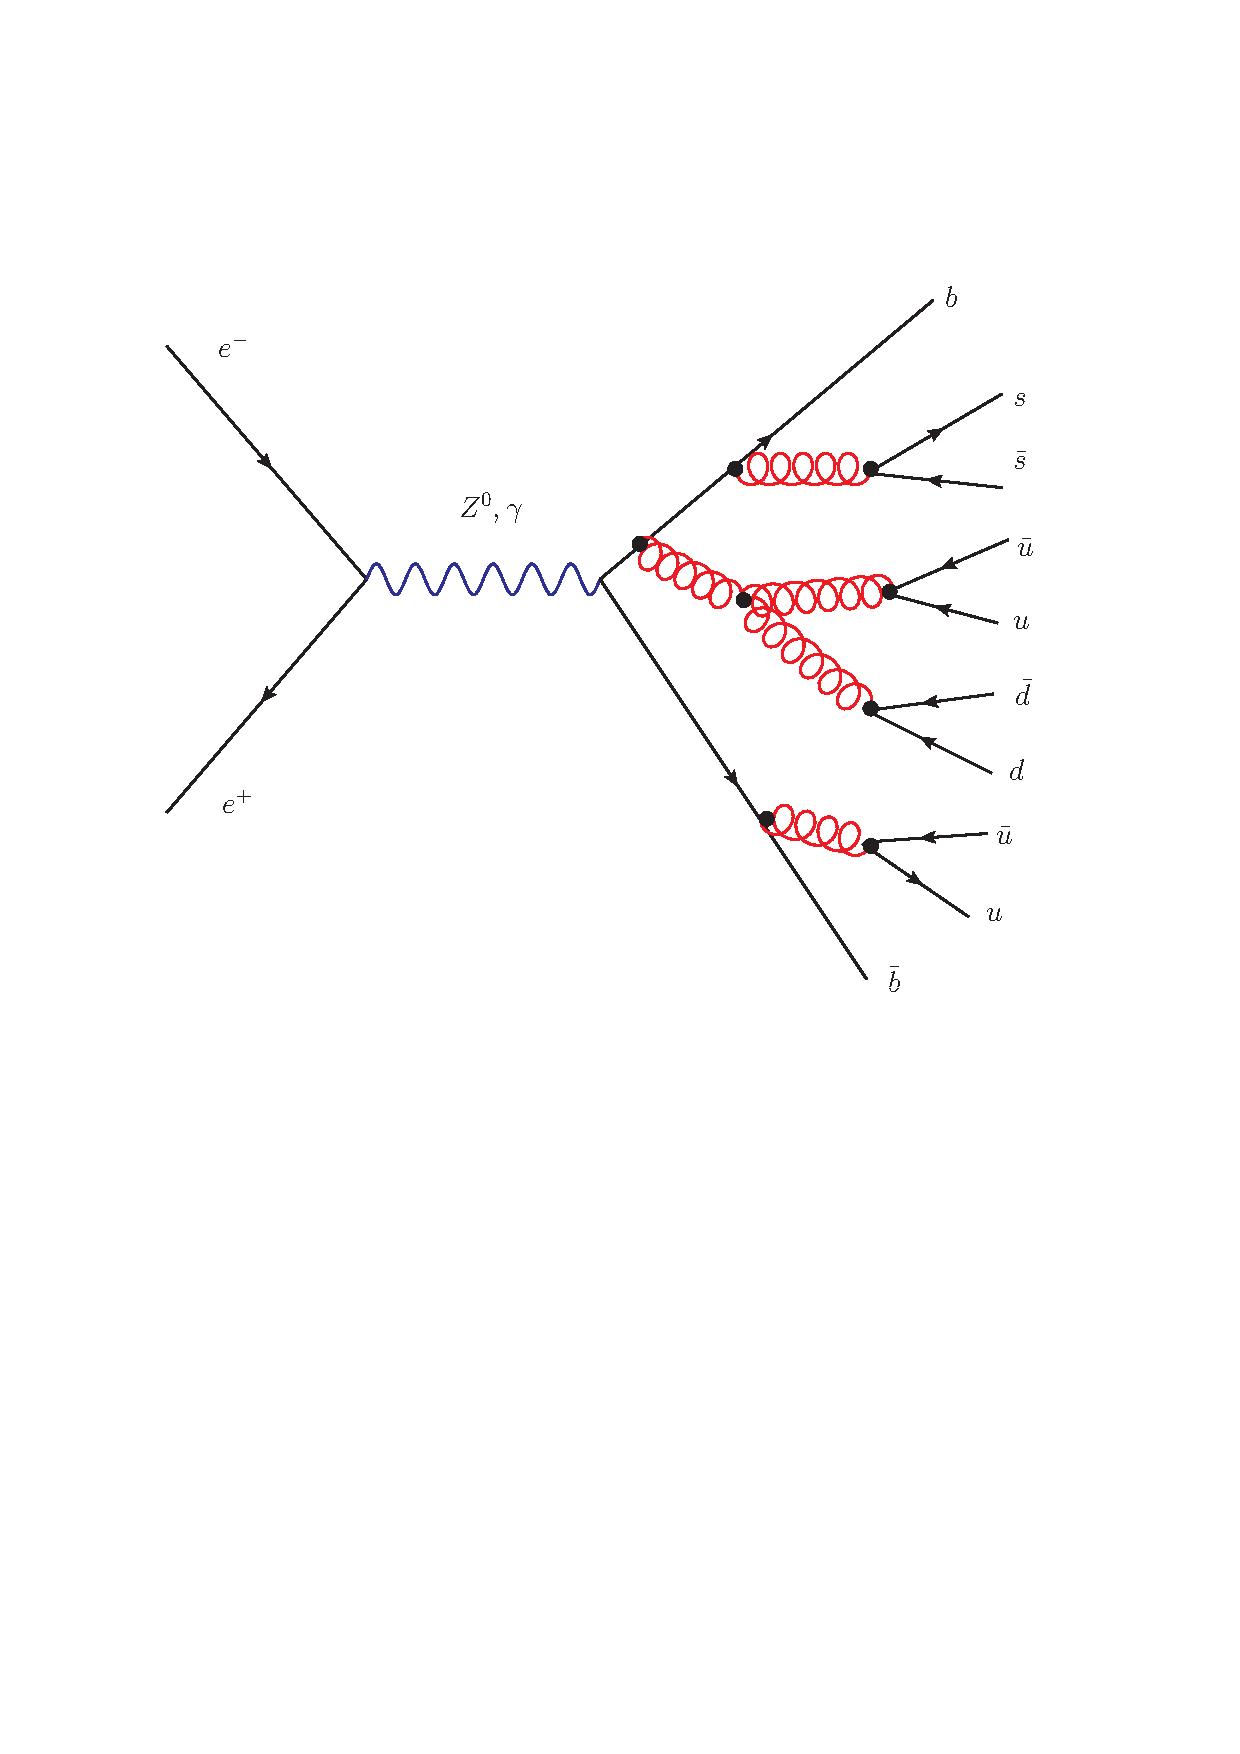
\includegraphics[width=0.8\linewidth]{figures/hadrons}
    \caption{This is process is the so called \textit{fragmentation}, in which a initial quark antiquark pair disolves into
further quark anti quark pairs ($\rightarrow$ quark confinement), absorbing the initial kinetic energy into mass. This will
continue until the momentum of individual quarks is small enough for going into bound states. Most often we will see two
jets, going into different directions. At very high energies, such as in our experiment, there is the possibility that
also non-virtual gluons will be created, resulting into more than two jets.}
    \label{fig:hadrons}
\end{figure}

\subsection{Bhabha scattering}
\label{sub:bhabha}
The process $e^+e^-\rightarrow e^+ e^-$ is called \textit{Bhabha scattering} and should be analyzed separately, since its
contribution play an important role in the further progress of the analysis. The reason for the difficulty in this process
is the occurrence of additional Feynman diagrams to be evaluated. If we separate the different contributions in specific  
channels with respect to the mandelstam variables\footnote{These lorentz-invariant variables are defined by 
\begin{align*}
s=(p_1+p_2)^2=(p_3+p_4)^2 \\
t=(p_1-p_3)^2=(p_2-p_4)^2 \\
u=(p_1-p_4)^2=(p_2-p_3)^2
\end{align*}
with the momenta $p_1$,$p_2$ of incoming and $p_3$ , $p_4$ of outgoing particles.
}, 
then we notice that we get additional contributions in the
t-channel, while in the processes treated until now only the s-channel contributed (see figure~\ref{fig:bhabha} for the
Feynman diagrams of the t-channel). The contributions for the $Z^0$ gauge boson only arise from the s-channel. Hence, if we
want to analyze the cross section of the s-channel, we need to subtract the t-channel. They differ with respect to the
angle $\theta$ between incoming and outgoing particles (at the peak $E=91GeV$):
\begin{align} 
  \mathrm{t-channel:}\quad    &\frac{d\sigma}{d\Omega} \sim \frac{(1+\cos\theta)^2}{(1-\cos \theta)^2}\\
  \mathrm{s-channel:}\quad    &\frac{d\sigma}{d\Omega} \sim (1+\cos^2\theta)
\end{align}
In the evaluation of the data we will take care to subtract the t-channel, in order to get the right result.

\begin{figure}[htpb]
    \centering
    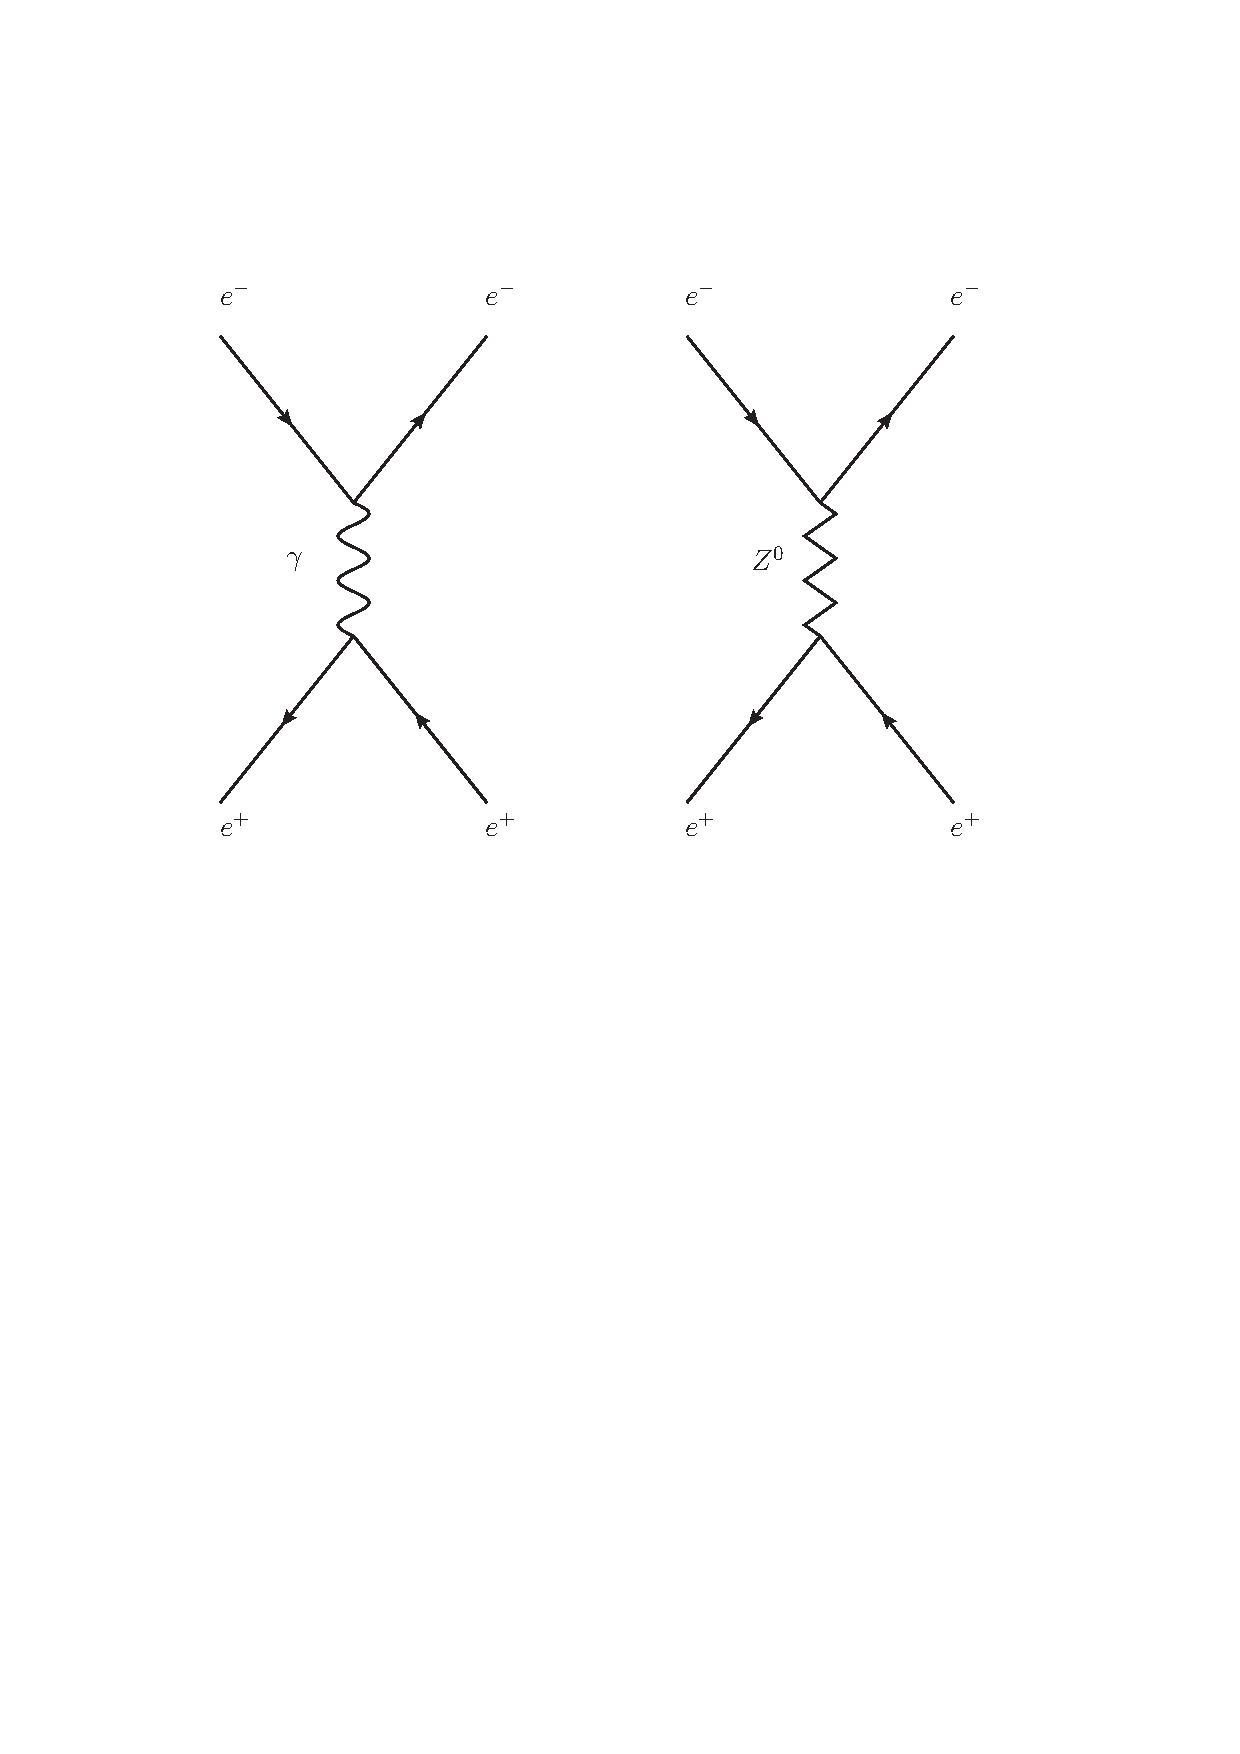
\includegraphics[width=0.6\linewidth]{figures/bhabha}
    \caption{T-channel of \textit{Bhabha scattering} $e^+e^-\rightarrow e^+ e^-$.}
    \label{fig:bhabha}
\end{figure}

\subsection{Cross sections and luminosity}
In the experiment, we will not be able to measure the cross section directly. We will arrive at this quantity by using our
counting the number of particles and inferring our knowledge about the collider (focus of the beam, orbital frequency). This
knowledge is condensed in the Quantity $\mathcal{L}$, the \textit{luminosity}, which we have to integrate over the collision:
\begin{equation}
    \sigma = \frac{N}{\int \mathcal{L} dt} + \kappa
\end{equation}
The $\int \mathcal{L} dt$ is called \textit{integrated luminosity} and $\kappa$ is the radiation correction coming from the
specifications of the collider.
\subsection{Cross-sections}
\label{sub:cross_sections}
In order to bring order into the rather theoretical description until now, we will list all decay widths by \eqref{eq:gamma_f},
following~\cite{ver}.
The electroweak force is split into the part of vector and axialvector coupling. 
\begin{align*}
    \Gamma_f &= \frac{\sqrt{2} G_f M_Z^3 N_c^f}{12 \pi} \left[ g_V^{f2} + g_A^{f2} \right] \\
       g_V^f &= I_3^f - 2 Q_f \sin^2 \theta_W \\
       g_A^f &= I_3^f \\
\Rightarrow \Gamma_f &= \frac{\sqrt{2} G_f M_Z^3 N_c^f}{12 \pi} \left[ (I_3^f - 2 Q_f \sin^2 \theta_W)^2 + (I_3^f)^2  \right] 
\end{align*}
Where we have used the following constants~\cite{pdg} (The last digit in brackets denotes to the uncertainty):
\begin{align*}
\label{eq:consts}
    N_c^f &= \text{color factor, one for leptons, three for quarks}  \\
    G_F &= 1.66387(6) \cdot 10^{-5} \mathrm{GeV^{-2}} \text{ Fermi coupling constant} \\
    M_Z &= 91.1876(21) \mathrm{GeV /c^{2}} \quad \mathrm{Z^0 \: boson \: mass} \\
    Q_f &= \text{ Electric charge in units of elementary charges}
\end{align*}
Using this formula, we arrive at the following decay widths:

\begin{align*}
    \Gamma_e = \Gamma_\mu = \Gamma_\tau &= 83.4 \: \mathrm{MeV}   \\
    \Gamma_{\nu_e} = \Gamma_{\nu_\mu} = \Gamma_{\nu_\tau} &= 166 \: \mathrm{MeV}  \\
    \Gamma_u = \Gamma_c &= 297 \: \mathrm{MeV} \\
    \Gamma_d = \Gamma_s = \Gamma_b &= 383 \: \mathrm{MeV} 
\end{align*}
Summing those up we arrive at the species dependent widths:
\begin{align*}
    \Gamma_{\mathrm{charged \: leptons}} = \Gamma_e + \Gamma_\mu + \Gamma_\tau &= 250\: \mathrm{MeV} \\
    \Gamma_{\mathrm{neutral \: leptons}} = \Gamma_{\nu_e} + \Gamma_{\nu_\mu} + \Gamma_{\nu_\tau} &= 498 \: \mathrm{MeV} \\
    \Gamma_{\mathrm{hadrons}} = \Gamma_u + \Gamma_d + \Gamma_b + \Gamma_c + \Gamma_s &= 1742 \: \mathrm{MeV} 
\end{align*}
Hence we arrive for the theoretical width of the $\mathrm{Z^0}$ boson:
\begin{equation*}
    \Gamma_Z = \Gamma_{\mathrm{charged \: leptons}} + \Gamma_{\mathrm{neutral \: leptons}}  + \Gamma_{\mathrm{hadrons}} = 2489 \: \mathrm{MeV}
\end{equation*}
Since the cross-section take the form \eqref{eq:breitwigner}, we can calculate its height at the maximum ($s = M_Z^2$) with
\begin{equation*}
    \sigma_f^{\mathrm{peak}} = \frac{12\pi \Gamma_e \Gamma_f }{M_Z^2 \Gamma_Z^2}
\end{equation*}
Our calculations yield
\begin{align*}
     \label{eq:peaks}
     \sigma_e = \sigma_\mu = \sigma_\tau &= 1.98 \: \mathrm{nb} \\
     \sigma_{\nu_e} = \sigma_{\nu_\mu} = \sigma_{\nu_\tau} &= 3.94 \: \mathrm{nb} \\
     \sigma_u = \sigma_c &= 7.05 \: \mathrm{nb} \\
     \sigma_d = \sigma_s = \sigma_b &= 9.09\: \mathrm{nb} 
    \end{align*}
 One might ask, how much the width of the $\mathrm{Z^0}$ boson would change if there was another fermion pair:
 \begin{equation*}
 \Gamma_{Z, \mathrm{new}} = 2655 \: \mathrm{MeV} \Rightarrow +7\% \: \text{larger}
 \end{equation*}
\subsubsection{Lepton universality}
\label{sub:lepton_universality}
As we already found in the section before, the decay widths of the leptons are identical in our model. The reason for this
\textbf{lepton universality} lies in the flavour independence of the theory, e.g.\ the gauge bosons (interactions are the same).
This theoretical prediction was confirmed at various experiments, including \textbf{LEP}.

\subsubsection{Number of neutrino generations}
\label{sub:number_of_neutrino_generations}
Until here we also assumed a definite number of three neutrino generations, originating from the close connection to the
lepton family, but this is not a trivial connection. Hence we can use this experiment as well to check if there were not
more than three neutrino generations (which would yield to inconsistencies in the standard model and the need for an theoretical
adjustment). As it turns out the number of neutrino generations predicted by the standard model is confirmed within all 
experimental data.

\subsubsection{Forward backward asymmetry}
\label{sub:forward_backward_asymmetry}
The asymmetry is defined to be
\begin{equation}
    \label{eq:asymmetry}
    A^f_{FB} = \frac{\int_0^1 \frac{d\sigma}{d\cos \theta}d\cos \theta - \int_{-1}^0 \frac{d\sigma}{d\cos \theta}d\cos \theta
        }{\int_0^1 \frac{d\sigma}{d\cos \theta}d\cos \theta 
    + \int_{-1}^0 \frac{d\sigma}{d\cos \theta}d\cos \theta}.
\end{equation}
The differential cross-section $\frac{d\sigma}{d\cos \theta}$ can be calculated with the \textsc{Born} approximation
\begin{equation}
    \frac{d\sigma}{d\cos \theta} = \frac{\pi \alpha^2 N_c^f}{2s} \left[ F_1(s) (1 + \cos^2 \theta) + 2 F_2(s) \cos\theta \right].
\end{equation}
The functions $F_1(s)$ and $F_2(s)$ can be calculated exactly, but they will not be shown here, as we will not need them
later (see \cite{ver} for their formulation). Hence the asymmetry \eqref{eq:asymmetry} yields the following result:
    \begin{align*}
        \label{eq:afb}
        \int \frac{d\sigma}{d\cos \theta}d\cos \theta &= \frac{\pi \alpha^2 N_c^f}{2s} 
        \left[ \frac{F_1(s)}{3} \cos^3 \theta + F_2(s) \cos^2\theta \right] + \mathrm{const}. \\
    \Rightarrow A_{FB}^f &= \frac{3 F_2}{4 F_1}
    \end{align*}
The asymmetry is the result of interference between the involved interactions. 

\subsection{Monte Carlo simulation}
\label{sub:monte_carlo_simulation}
%todo


